\section{Техническое задание}
\subsection{Основание для разработки}

Основанием для разработки является задание на выпускную квалификационную работу бакалавра <"Платформа для создания компьютерных изометрических ролевых игр с заранее отрисованным двухмерным фоном и спрайтовыми персонажами">.

\subsection{Цель и назначение разработки}

Основной задачей выпускной квалификационной работы является разработка платформы для создания компьютерных изометрических ролевых игр с заранее отрисованным двумерным фоном и спрайтовыми персонажами для продвижения популярности рпг-игр».

Данный программный продукт предназначен для демонстрации практических навыков, полученных в течение обучения. Исходя из этого, основную цель предлагается рассмотреть в разрезе двух групп подцелей.

Задачами данной разработки являются:
\begin{itemize}
\item проектирование интерфейса;
\item разработка архитектуры приложения;
\item проектирование игровых сценариев;
\item реализация взаимодействия приложения с пользователем;
\item реализация графики приложения;
\end{itemize}

\subsection{Требования пользователя к платформе}

платформа должна включать в себя:
\begin{itemize}
    \item создание зон.
    \item создание объектов.
    \item создание персонажей.
    \item добавление объектов в зону.
    \item удаление объектов из зоны.
    \item реализацию сценариев.
\end{itemize}

Композиция шаблона игры, созданной на движке, представлена на рисунке ~\ref{maket:image}.

\begin{figure}[ht]
	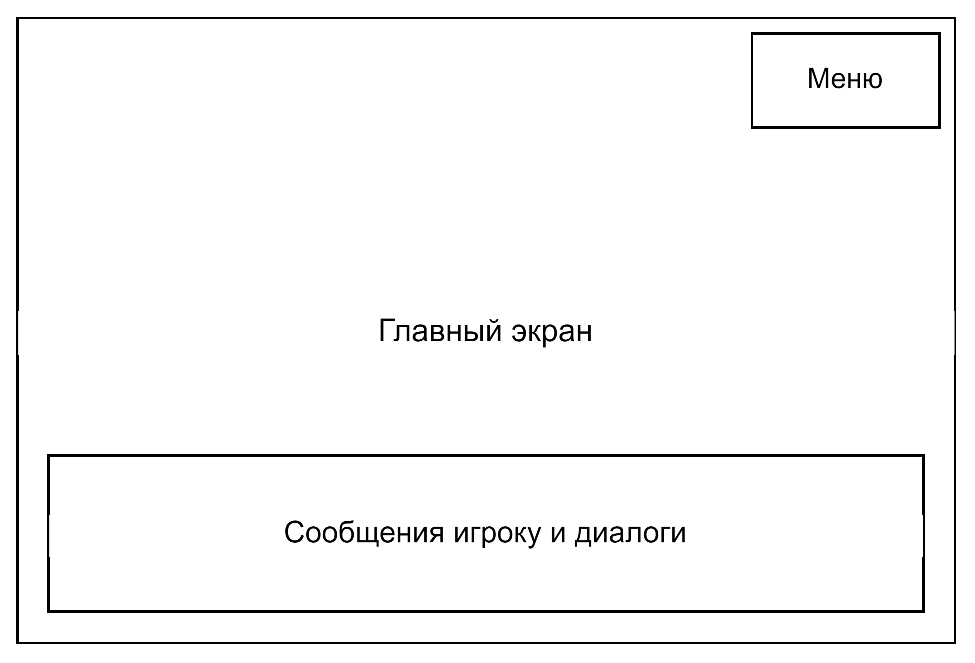
\includegraphics[width=1\linewidth]{maket}
	\caption{Композиция шаблона интерфейса игры}
	\label{maket:image}
\end{figure}
%\vspace{-\figureaboveskip} % двойной отступ не нужен (можно использовать, если раздел заканчивается картинкой)

\subsection{Пример игры}
 \begin{itemize}
 	\item ролевая игра моделирует все основные механики Dungeons and Dragons, в которой игрок управляет персонажем, который бродит по одноуровневому подземелью, собирая сокровища и убивая монстров. Подземелье визуализируется в двухмерном виде сверху с использованием экранной графики персонажей и управляется с помощью команд с мыши. Подземелье имеет фиксированную планировку, но встречи с монстрами и сокровища генерируются заданным образом.
 	\begin{itemize}
 		\item 1. Цель игры: Основная цель игры заключается в исследовании мира, выполнении заданий и квестов, сражении с врагами и развитии своего персонажа. Игра также имеет главный сюжет, который игрок может прогрессировать, следуя определенным событиям и заданиям
 		\item 2. Боевая система:  Бои могут происходить в режиме реального времени. Игрок может управлять группой персонажей и давать им команды в бою. В бою игрок может использовать различные атаки, заклинания и способности своего персонажа для победы над врагами
 		\item 3. Персонажи: Игрок может создать своего уникального персонажа, выбрав класс, расу, навыки и характеристики. Каждый класс имеет свои особенности и специализации, определяющие стиль игры и возможности персонажа. Персонажи могут повышать уровень, получать новые навыки и способности, улучшать характеристики и собирать экипировки
 		\item 4. Исследование мира: Игрок может свободно перемещаться по миру игры, исследуя различные локации и взаимодействуя с окружающими объектами. Во время исследования игрок может встретить неигровых персонажей (NPC), с которыми можно общаться, получать задания и информацию о мире.
 		\item 5. Прогрессия и развитие: Игрок может зарабатывать опыт и повышать уровень своего персонажа. Повышение уровня позволяет персонажу получать новые навыки, улучшать характеристики и получать новые способности. Игрок также может собирать и улучшать экипировку для своего персонажа, чтобы повысить его силу и выживаемость.
 		\item 6. Задания и квесты: Игрок может выполнять различные задания и квесты, предлагаемые неигровыми персонажами. Задания могут включать поиск предметов, убийство определенных врагов, решение головоломок и т.д. За выполнение заданий игрок может получать награды, опыт и продвигаться в сюжете игры.
 	\end{itemize}
 \end{itemize}
 
\subsection{Особенности Dungeons and Dragons}
\begin{itemize}
	\item Dungeons and Dragons (DnD) - это настольная ролевая игра, в которой игроки сотрудничают вместе, чтобы создать историю в фантастическом мире. В DnD один игрок выступает в роли Мастера игры (Мастера подземелий), который рассказывает и контролирует мир, а остальные игроки играют за своих персонажей, которых они создают и развивают.
	\begin{itemize} Основные элементы ролевой системы DnD включают:
		\item 1. Классы и расы: Классы представляют различные роли и специализации персонажей, такие как воин, маг, жрец. Каждый класс имеет свои уникальные способности и навыки.
			\begin{itemize}
				\item Особенности воина: воин специализируется на ближнем бою, может использовать все виды оружия, может носить все доспехи и щиты, не способен накладывать заклинания, его кость здоровья 10-гранный кубик (D10).
				\item Особенности мага: маг специализируется на дальнем бою, может использовать только боевые посохи и короткие мечи, не может носить доспехи , способен накладывать заклинания, наносящие большое количество урона, его кость здоровья 6-гранный кубик (D6).
				\item Особенности жреца: жрец специализируется на ближнем бою, может использовать простое оружия, может носить лёгкие,средние доспехи и щиты, способен накладывать заклинания, исцеляющие его, его кость здоровья 8-гранный кубик (D8).
			\end{itemize}

		\item Расы определяют происхождение персонажа и дают особые характеристики и способности. Примеры рас включают эльфов, дварфов, людей.
			\begin{itemize}
			\item Особенности человека: человек на старте получает +1 ко всем характеристикам, его размер средний.
			\item Особенности эльфа: эльф получает +2 к ловкости и +1 к мудрости, его размер средний, у эльфа есть тёмное зрение в радиусе 30 футов.
			\item Особенности дварфа: дварф получает +2 к силе и +2 к телосложению, его размер маленький, у дварфа есть тёмное зрение в радиусе 30 футов.
			\end{itemize}
		\item 2. Характеристики:
		\begin{itemize}
			\item Характеристики определяют физические и умственные способности персонажа, такие как сила, ловкость, телосложение, интеллект, мудрость, харизма. Они влияют на способности и успех персонажа в различных ситуациях.
			\item Сила - характеристика влияющая на броски атак рукопашным оружием, а так же на проверки навыков: атлетика.
			\item Ловкость - характеристика влияющая на броски атак совершаемых стрелковым оружием, на класс доспеха персонажа, а так же на проверки навыков: акробатика, ловкость рук, скрытность.
			\item Телосложение - характеристика влияющая на колличество здоровья персонажа.
			\item Интеллект - характеристика влияющая на броски атак совершённых заклинаниями волшебника, а так же на проверки навыков: магия, история, природа, расследование, религия.
			\item Мудрость - характеристика влияющая на броски атак  совершённых заклинаниями жреца, а так же на проверки навыков: восприятие, выживание, проницательность, уход за животными, медицина.
			\item Харизма - характеристика влияющая на общение с не игровыми персонажами, а так же на проверки навыков: выступление, убеждение, обман, запугивание.
		\end{itemize}
		\item 3. Навыки:
		\begin{itemize}
			\item Навыки представляют специализации персонажа в определенных областях, таких как взлом замков, обращение с оружием, магия и т.д. Навыки могут быть использованы для выполнения действий и решения задач
		\end{itemize}
		\item 4. Броски костей:
		\begin{itemize}
			\item Игра DnD использует различные виды игровых костей для случайной генерации результатов. Например, для определения успеха атаки или проверки навыка игрок может бросить 20-гранный кубик (D20) и добавить соответствующие модификаторы.
		\end{itemize}
		\item 5. Приключения и задания:
		\begin{itemize}
			\item Мастер игры создает историю, включающую задания и приключения, которые игроки выполняют. Задания могут включать исследование подземелий, сражение с монстрами, решение головоломок и взаимодействие с неигровыми персонажами.
		\end{itemize}
		\item 6: Прогрессия и опыт:
		\begin{itemize}
			\item Персонажи получают опыт за выполнение заданий и сражение с врагами. Зарабатывая опыт, персонажи повышают уровень, получают новые способности и становятся сильнее.
		\end{itemize}
		\item 7. Магия:
		\begin{itemize}
			\item DnD имеет разветвленную систему магии, позволяющую персонажам использовать заклинания различных уровней и школ. Магические заклинания могут влиять на бой, лечение, обнаружение и другие аспекты игры.
		\end{itemize}
	\end{itemize}
\end{itemize}

\subsection{Интерфейс пользователя}
Создаётся рабочее окно tkinter, на нём пользователь видит текущую зону, из зоны current\_area, так же все объекты, находящиеся в ней, и всех персонажей из команды персонажей, текущей игры. Пользователь может взаимодействовать с окном с помощью мыши. Левым кликом мыши по окну вызывает метод mouse\_click у текущей игры. который вызывает проверку находится ли в координатах, в которых был совершён клик, какой-либо персонаж или объект, и если есть, то вызвать метод on\_click. Если персонажа в данных координатах нет, то вызвать у всех персонажей с полем category == "pc" метод search\_position(x,y), который указывает координаты движения, которые должны прийти персонажи. Так же работают все сценарии, конкретной зоны. они работают до тех пор, пока не будет вызвано условие останавливающее, конкретный сценарий.
\subsection{ Моделирование вариантов использования}
На основании анализа предметной области в программе должны быть реализованы следующие прецеденты:
\begin{enumerate}
\item Создание персонажа.
\item Создание зоны.
\item Создание объекта.
\item Удаление объекта.
\item Создание сценария.
\item Удаление сценария.
\end{enumerate}
Таким образом, на рисунке ~\ref{prec:image}сформированы следующие действия пользователя и их последствия.
\begin{figure}[ht]
	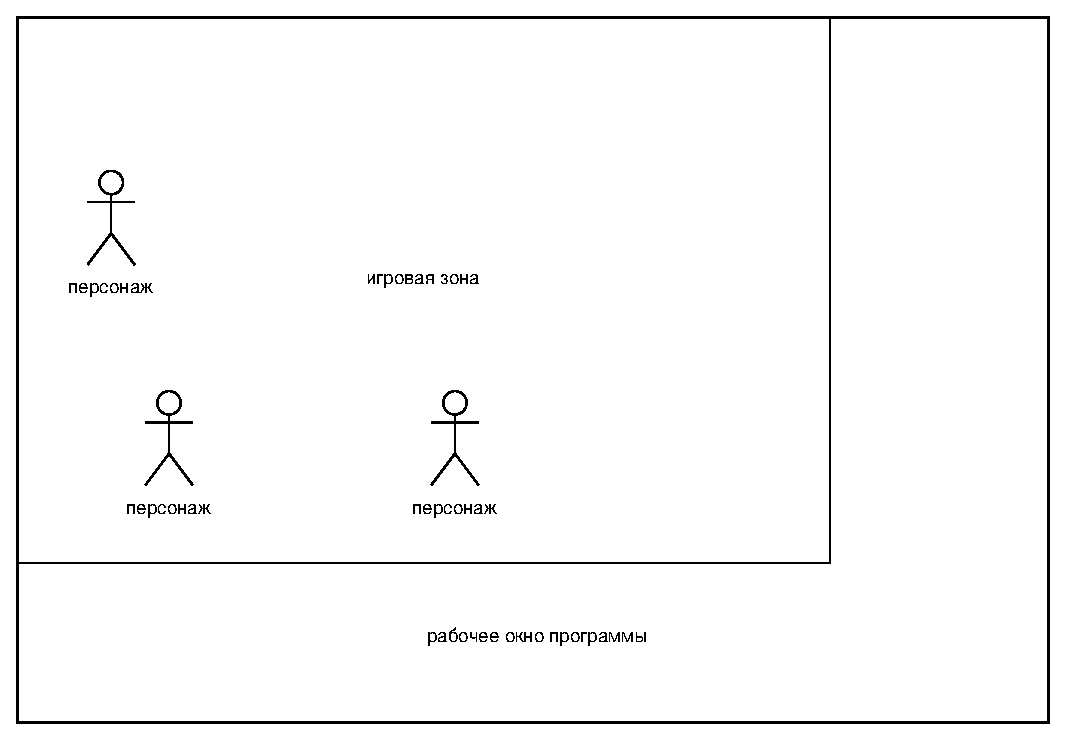
\includegraphics[width=1\linewidth]{prec}
	\caption{Шаблон интерфейса игры}
	\label{prec:image}
\end{figure}
%\vspace{-\figureaboveskip} % двойной отступ не нужен (можно использовать, если раздел заканчивается картинкой)

\subsection{Требования к оформлению документации}

Разработка программной документации и программного изделия должна производиться согласно ГОСТ 19.102-77 и ГОСТ 34.601-90. Единая система программной документации.
